\documentclass[superscriptaddress,10pt,prl,floatfix,nofootinbib,aps]{revtex4-2} 

\newif\ifsupp
\supptrue   % set \suppfalse for submission (main only)

\usepackage[labeled]{multibib}
\usepackage{hyperref}
\usepackage{xr-hyper}
\externaldocument{main}

\usepackage[scaled]{helvet}
\renewcommand{\familydefault}{\sfdefault}

\input{glyphtounicode}
\pdfgentounicode=1
\usepackage[T1]{fontenc}
\usepackage[utf8]{inputenc}
\usepackage[english]{babel}
\usepackage{amsmath}  % needed for \tfrac, \bmatrix, etc.
\usepackage{amsfonts} % needed for bold Greek, Fraktur, and blackboard bold
\usepackage{amssymb}
\usepackage{graphicx} % needed for figures
\usepackage{float}  % Add in your preamble
\usepackage[table]{xcolor}
% \usepackage{xcolor}
\usepackage{placeins}
\usepackage{newfloat}

\usepackage{lineno}
\usepackage{caption}

\DeclareFloatingEnvironment[name={\textbf{Supplementary Figure}}]{suppfigure}

\newcommand{\aref}[1]{\hyperref[#1]{Appendix~\ref*{#1}}}
\DeclareCaptionLabelSeparator{line}{\hspace{2pt}\bf{|}\hspace{2pt}}

\DeclareFloatingEnvironment[name={\textbf{Supplementary Table}}]{supptable}
\renewcommand{\thesupptable}{S\arabic{supptable}}

\begin{document}

\setcounter{page}{1}
\pagenumbering{roman}
\begin{center}
{\LARGE \textbf{Supplementary Information}}
\end{center}

\begin{center}
{Eight-Qubit Operation of a 300 mm SiMOS Foundry-Fabricated Device}
\end{center}
\FloatBarrier

\begin{suppfigure*}
    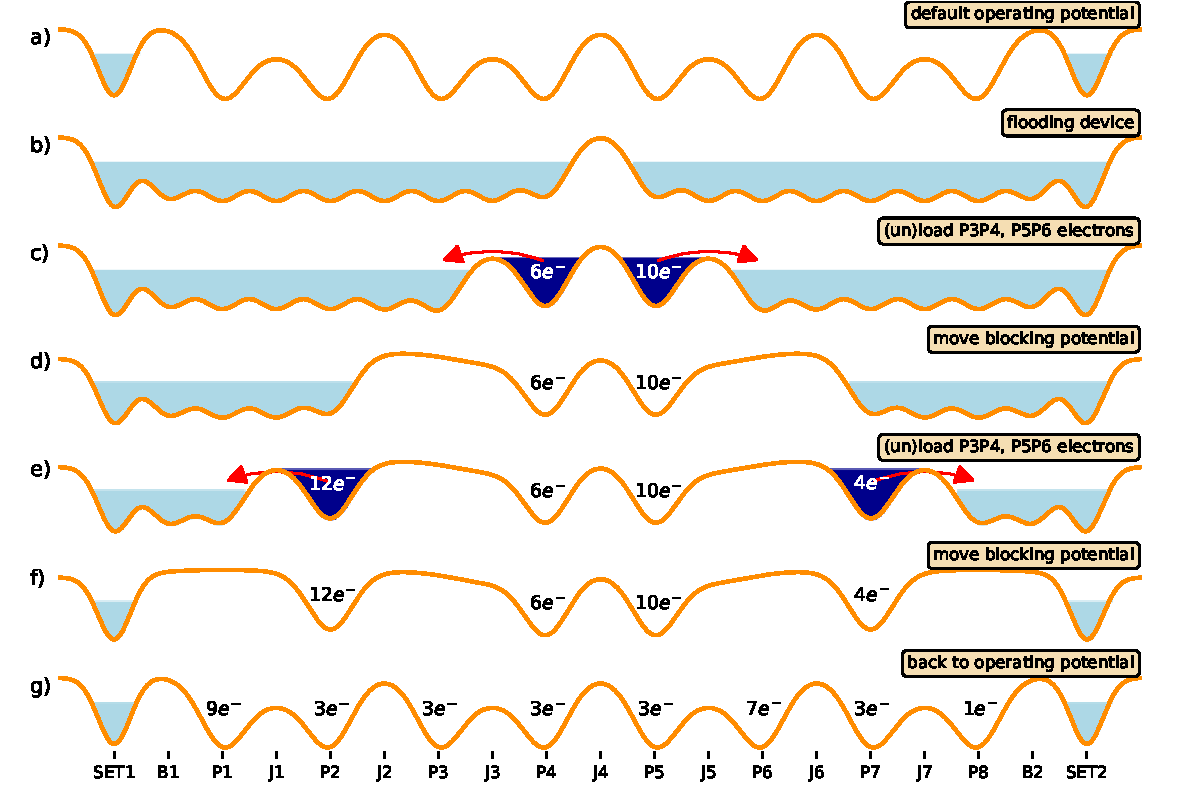
\includegraphics[width=0.8\textwidth, angle = 0]{loading_sequence.pdf} % rabis.pdf
    \caption{
        \textbf{Electron loading sequence of the entire device.} 
        \textbf{a)} Initial DC operating potential.
        \textbf{b)} Flooding the device from both sides with a 2-dimensional electron gas from the SET islands symmetric around J4.
        \textbf{c)} Set calibrated loading voltages (P4, P5) and barrier voltages (J4, J5) to reduce the Fermi sea to the desired integer of electrons.
        \textbf{d)} Electrons are trapped to central dots by applying blocking potentials (J2, P3, J3 and J5, P6, J6).
        \textbf{e)} Similar to (c) but in lateral dots, loading voltages (P2 and P7) and barrier voltages (J1 and J7).
        \textbf{f)} Similar to (d) blocking potentials to trap electrons under P2 and P7 while pushing out the Fermi sea.
        \textbf{g)} Returning to the initial DC operating potential.
    }
    \label{supp:loading_sequence}
\end{suppfigure*}

\begin{suppfigure*}
    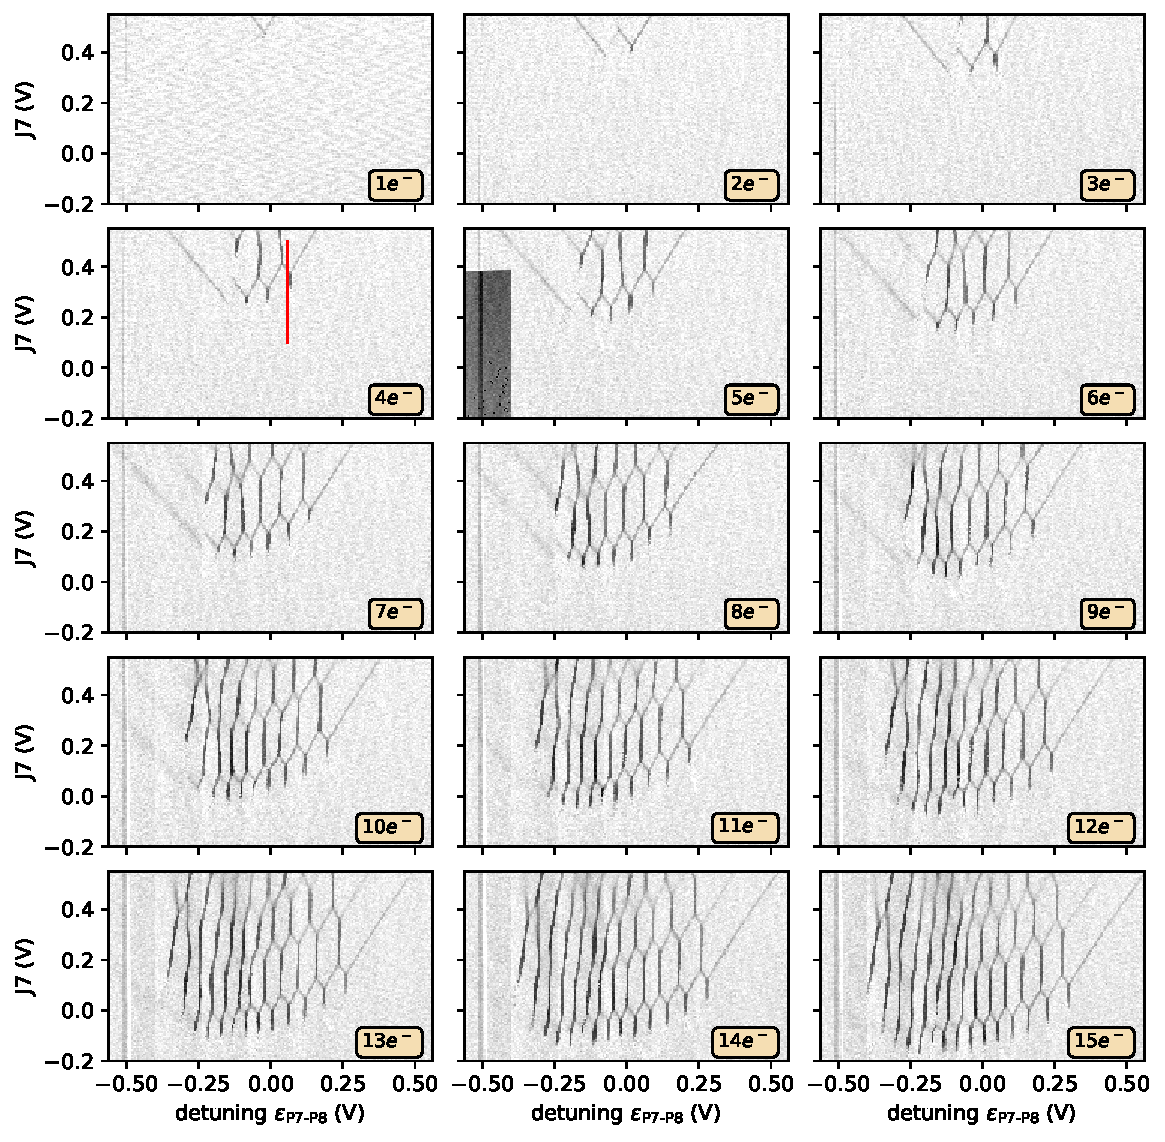
\includegraphics[width=0.9\textwidth, angle = 0]{e_loading.pdf} % rabis.pdf
    \caption{
        \textbf{Isolated mode stability maps of P7P8 DQD | }
        Electrons are incrementally loaded into the double dot using the technique shown in Supplementary Figure \ref{supp:loading_sequence}. 
        The higher the voltage of P7 during the sequence stop shown in Supplementary Figure \ref{supp:loading_sequence}e, the more electrons will be captured in P7--P8. The loading voltage decreases with an increased number of electrons per DQD~\cite{leon_coherent_2020}. Inter-dot transitions (vertical) are extending, following charge occupancy numbers, thus tunnel coupling among DQDs before forming a quantum dot under the intermediate J-gate is enhanced as more electrons are accumulated.
        The red line in the four electron maps indicates the scan shown in Supplementary Figure \ref{supp:ex_turonon}a.
    }
    \label{supp:e_loading}
\end{suppfigure*}

\begin{supptable}[h!]
\centering
\begin{tabular}{ | c | c | c | c |}
\hline
\textbf{P1P2} & \textbf{P3P4} & \textbf{P5P6} & \textbf{P7P8}\\
\hline
\cellcolor{yellow} (3-3) & \cellcolor{green} (3-3) & \cellcolor{red!30} (3-3) & \cellcolor{green} (3-1) \\
\cellcolor{yellow} (5-3) & \cellcolor{yellow} (5-3) & \cellcolor{yellow} (3-5) & \cellcolor{yellow}(3-3)\\
\cellcolor{green}(9-3) &                            & \cellcolor{green} (3-7) & \cellcolor{red!30}(5-3)\\
\cellcolor{red!30} (13-3) &  & & \\
\hline
\end{tabular}
\caption{Charge configurations examined in this measurement campaign for all double quantum dots. Green highlights indicate the used charge configuration per double dot in the main figure 1. Yellow highlights mark charge configurations that allowed the tuning of qubits which showed Rabi oscillations with lower Q-factors. Supplentary Fig. \ref{supp:other_charge_configs} shows some of the qubit results for the yellow charge configurations. Charge configurations in red yielded no qubits.}
\label{tab:other_change_configs}
\end{supptable}

\begin{suppfigure*}
    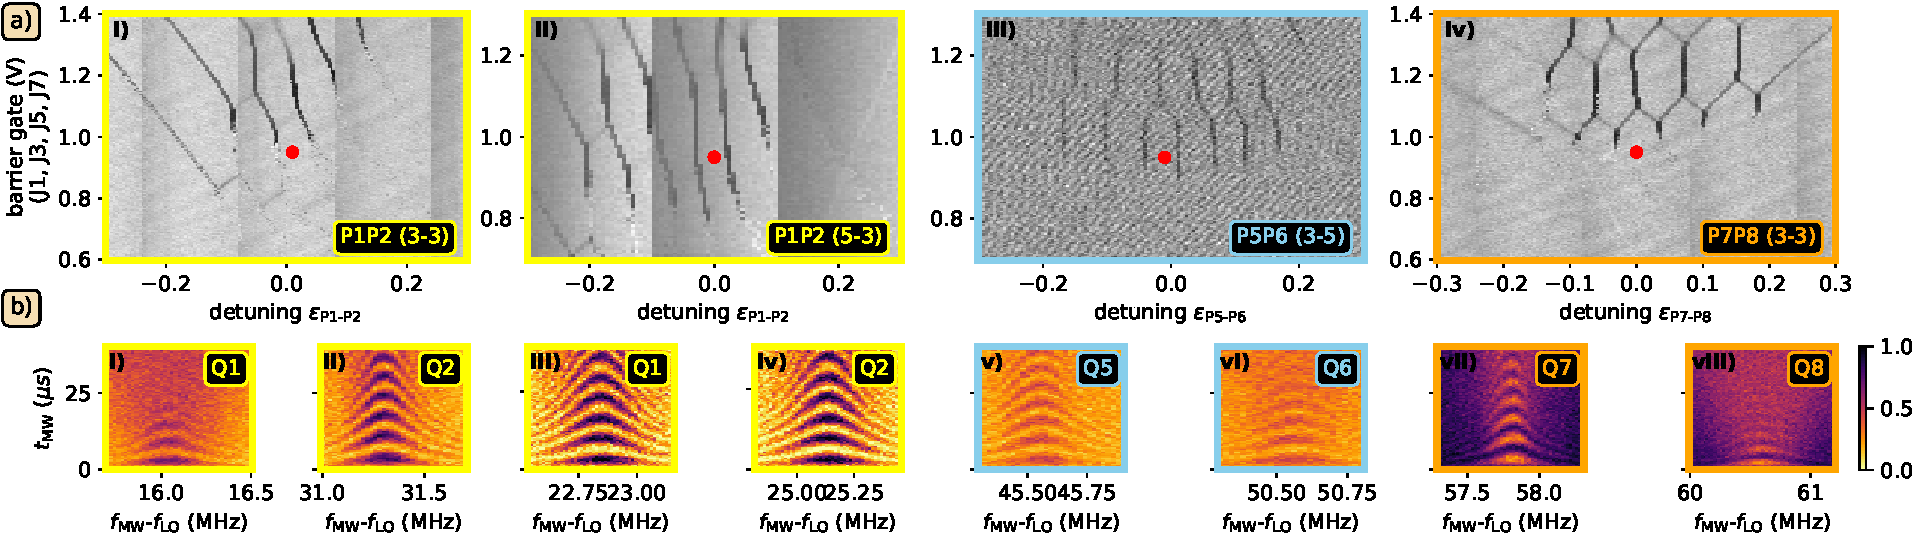
\includegraphics[width=\textwidth, angle = 0]{other_charge_configs.pdf} % rabis.pdf
    \caption{
        \textbf{Charge stability maps and Rabi-chevron measurement for different electron numbers |} 
        Red circles mark the charge
configuration used for the measured qubits.
        \textbf{P1-P2 (3-3):} a)i, b) i,ii
        \textbf{P1-P2 (5-3):} a)ii, b) iii,iv
        \textbf{P5-P6 (3-5):} a)iii, b) v,vi; Rabi chevrons were measured directly via SET2 without electron cascade, hence the low visibility
        \textbf{P7-P8 (3-3):} a)iv, b) vii,viii
    }
    \label{supp:other_charge_configs}
\end{suppfigure*}

\begin{suppfigure*}
    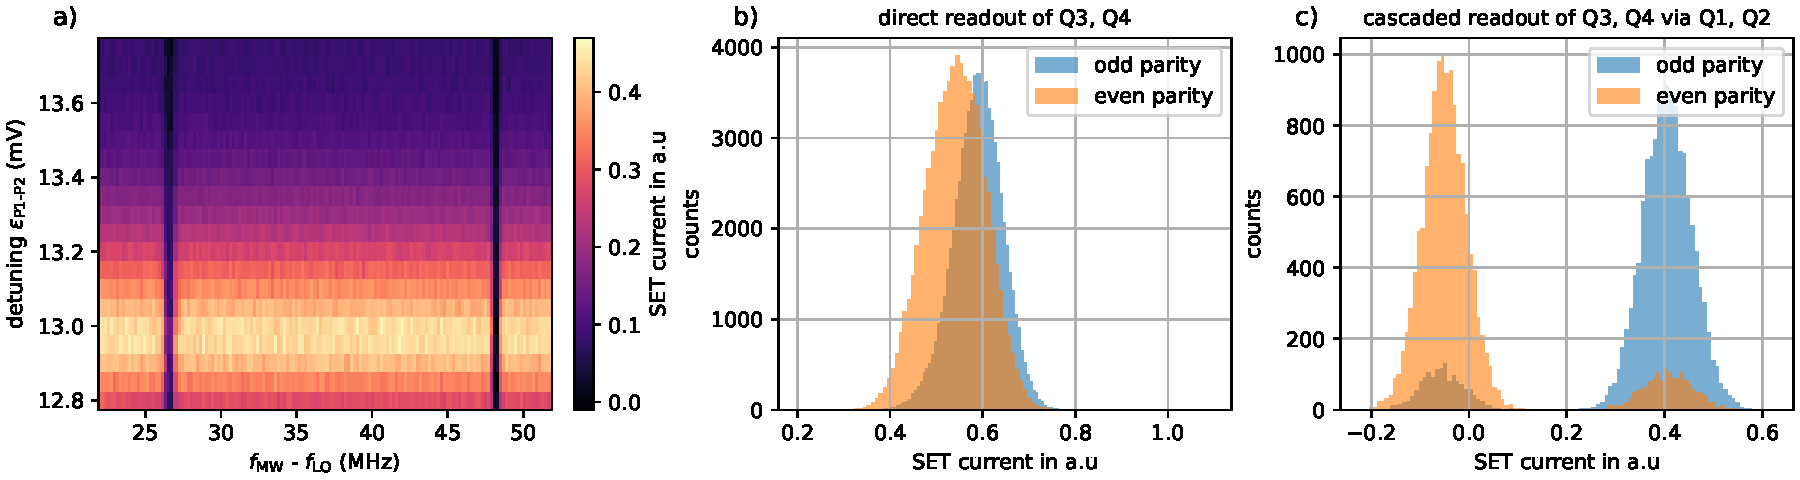
\includegraphics[width=0.9\textwidth, angle = 0]{cascading_calibration.pdf} % rabis.pdf
    \caption{
        \textbf{Calibration of cascaded readout | } 
        \textbf{a)} Difference in visibility of an ESR measurement when changing the detuning $\epsilon_{P1-P2}$. The high contrast region corresponds to a cascaded electron transition from P1 to P2
        \textbf{b)} Histograms of an ESR measurement using direct readout of P3P4 double dot
        \textbf{c)} Histograms of an ESR measurement using cascaded readout of P3P4 double dot via P1P2 cascading
    }
    \label{supp:cascading_calibration}
\end{suppfigure*}

\begin{suppfigure*}
    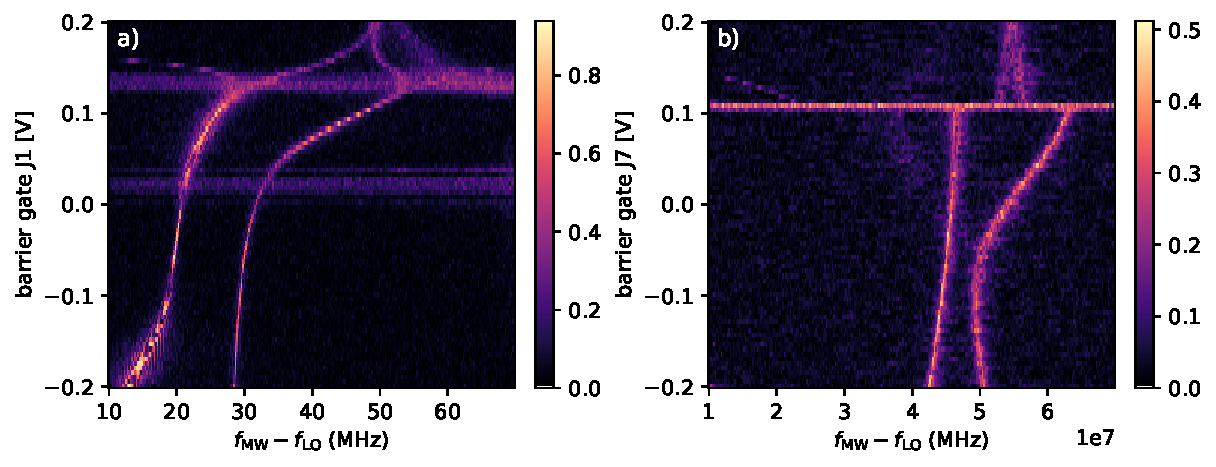
\includegraphics[width=0.65\textwidth, angle = 0]{ex_turnon.pdf} % rabis.pdf
    \caption{
        \textbf{Two qubit exchange | } ESR measurement vs barrier gate voltage in DQDs. Horizontal splitting in qubits ESR frequencies at high barrier gate voltage corresponds to their exchange coupling.
        \textbf{a)} P1P2, continuous exponential turn on of exchange through Heisenberg interaction at (9,3) charge configuration
        \textbf{b)} P7P8, sudden turn of exchange via shuttling to intermediate J-dot under J7 at (1,3) charge configuration. The corresponding charge stability map with 4 electrons can be seen in Supplementary Figure \ref{supp:e_loading}. The scan axis of the measurement shown here is indicated by the red line
    }
    \label{supp:ex_turonon}
\end{suppfigure*}

\begin{suppfigure*}
    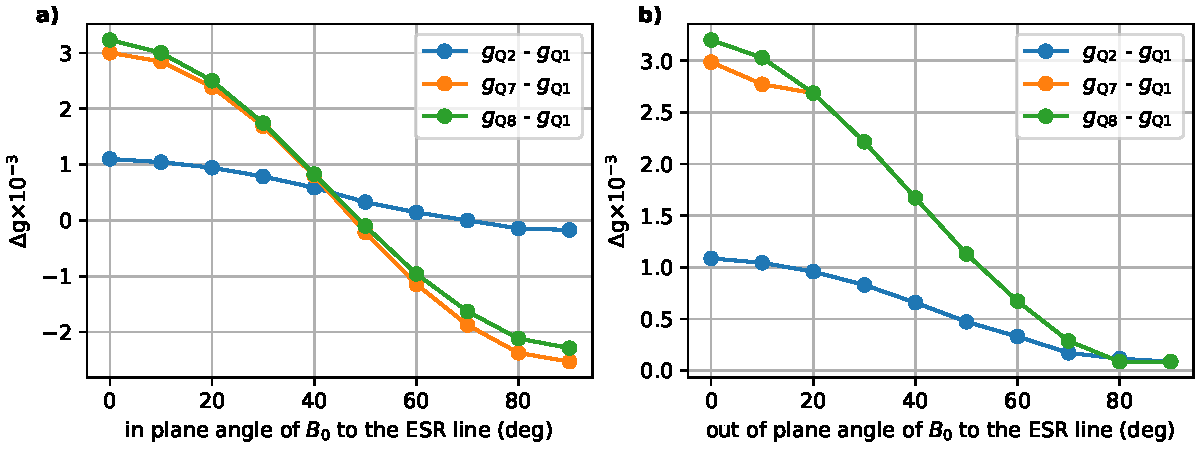
\includegraphics[width=0.65\textwidth, angle = 0]{b_field_angles.pdf}
    \caption{
        \textbf{Qubit Larmor frequencies vs magnetic field angle $B_0$| }
        \textbf{a)} rotation $\psi$ in the plane spanned by the qubit array and the normal to the schematic shown in Fig 1a. Rotation from [110] to [1$\bar{1}$0] ($45^{\circ}$)
        \textbf{b)} rotation $\theta$ in the plane depicted in schematic \ref{fig:mega_figure}a. Both angles being 0 results in $B_0$ pointing parallel to the qubit array. Rotation from [110] to [001]
    }
    \label{supp:b_field_rot}
\end{suppfigure*}

\begin{suppfigure*}
    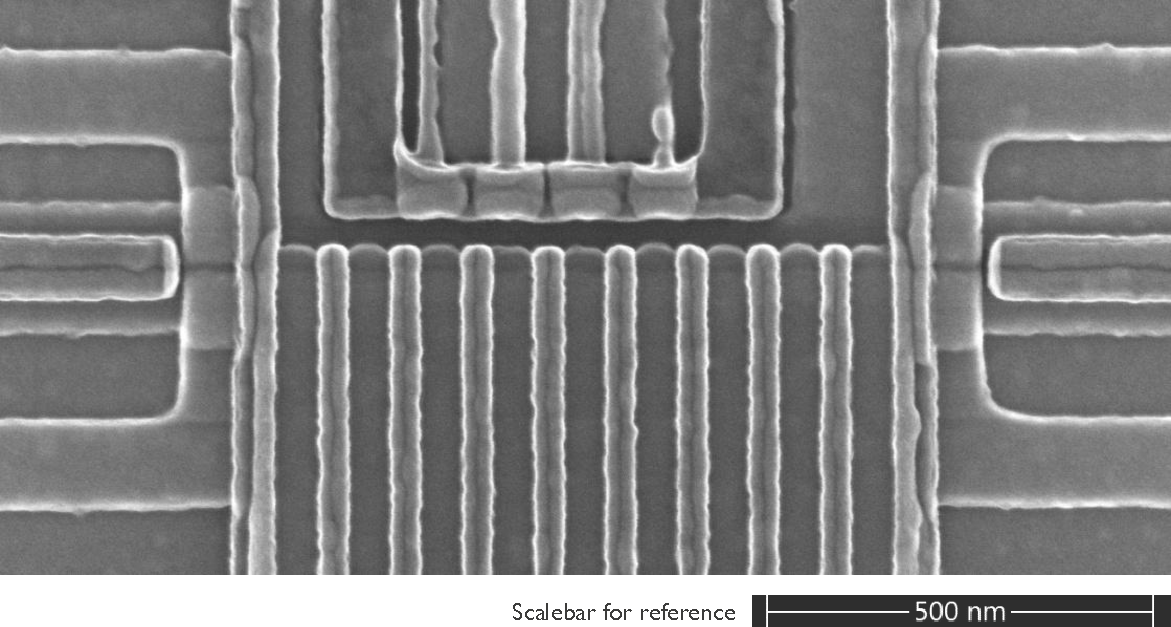
\includegraphics[width=0.5\textwidth, angle = 0]{SEM.pdf}
    \caption{
        \textbf{SEM image of a similar device} \cite{li_flexible_2021}
    }
    \label{supp:SEM}
\end{suppfigure*}


\FloatBarrier
\bibliography{8Qbib}

\end{document}